% Options for packages loaded elsewhere
\PassOptionsToPackage{unicode}{hyperref}
\PassOptionsToPackage{hyphens}{url}
%
\documentclass[
]{article}
\usepackage{amsmath,amssymb}
\usepackage{lmodern}
\usepackage{iftex}
\ifPDFTeX
  \usepackage[T1]{fontenc}
  \usepackage[utf8]{inputenc}
  \usepackage{textcomp} % provide euro and other symbols
\else % if luatex or xetex
  \usepackage{unicode-math}
  \defaultfontfeatures{Scale=MatchLowercase}
  \defaultfontfeatures[\rmfamily]{Ligatures=TeX,Scale=1}
\fi
% Use upquote if available, for straight quotes in verbatim environments
\IfFileExists{upquote.sty}{\usepackage{upquote}}{}
\IfFileExists{microtype.sty}{% use microtype if available
  \usepackage[]{microtype}
  \UseMicrotypeSet[protrusion]{basicmath} % disable protrusion for tt fonts
}{}
\makeatletter
\@ifundefined{KOMAClassName}{% if non-KOMA class
  \IfFileExists{parskip.sty}{%
    \usepackage{parskip}
  }{% else
    \setlength{\parindent}{0pt}
    \setlength{\parskip}{6pt plus 2pt minus 1pt}}
}{% if KOMA class
  \KOMAoptions{parskip=half}}
\makeatother
\usepackage{xcolor}
\usepackage[margin=1in]{geometry}
\usepackage{color}
\usepackage{fancyvrb}
\newcommand{\VerbBar}{|}
\newcommand{\VERB}{\Verb[commandchars=\\\{\}]}
\DefineVerbatimEnvironment{Highlighting}{Verbatim}{commandchars=\\\{\}}
% Add ',fontsize=\small' for more characters per line
\usepackage{framed}
\definecolor{shadecolor}{RGB}{248,248,248}
\newenvironment{Shaded}{\begin{snugshade}}{\end{snugshade}}
\newcommand{\AlertTok}[1]{\textcolor[rgb]{0.94,0.16,0.16}{#1}}
\newcommand{\AnnotationTok}[1]{\textcolor[rgb]{0.56,0.35,0.01}{\textbf{\textit{#1}}}}
\newcommand{\AttributeTok}[1]{\textcolor[rgb]{0.77,0.63,0.00}{#1}}
\newcommand{\BaseNTok}[1]{\textcolor[rgb]{0.00,0.00,0.81}{#1}}
\newcommand{\BuiltInTok}[1]{#1}
\newcommand{\CharTok}[1]{\textcolor[rgb]{0.31,0.60,0.02}{#1}}
\newcommand{\CommentTok}[1]{\textcolor[rgb]{0.56,0.35,0.01}{\textit{#1}}}
\newcommand{\CommentVarTok}[1]{\textcolor[rgb]{0.56,0.35,0.01}{\textbf{\textit{#1}}}}
\newcommand{\ConstantTok}[1]{\textcolor[rgb]{0.00,0.00,0.00}{#1}}
\newcommand{\ControlFlowTok}[1]{\textcolor[rgb]{0.13,0.29,0.53}{\textbf{#1}}}
\newcommand{\DataTypeTok}[1]{\textcolor[rgb]{0.13,0.29,0.53}{#1}}
\newcommand{\DecValTok}[1]{\textcolor[rgb]{0.00,0.00,0.81}{#1}}
\newcommand{\DocumentationTok}[1]{\textcolor[rgb]{0.56,0.35,0.01}{\textbf{\textit{#1}}}}
\newcommand{\ErrorTok}[1]{\textcolor[rgb]{0.64,0.00,0.00}{\textbf{#1}}}
\newcommand{\ExtensionTok}[1]{#1}
\newcommand{\FloatTok}[1]{\textcolor[rgb]{0.00,0.00,0.81}{#1}}
\newcommand{\FunctionTok}[1]{\textcolor[rgb]{0.00,0.00,0.00}{#1}}
\newcommand{\ImportTok}[1]{#1}
\newcommand{\InformationTok}[1]{\textcolor[rgb]{0.56,0.35,0.01}{\textbf{\textit{#1}}}}
\newcommand{\KeywordTok}[1]{\textcolor[rgb]{0.13,0.29,0.53}{\textbf{#1}}}
\newcommand{\NormalTok}[1]{#1}
\newcommand{\OperatorTok}[1]{\textcolor[rgb]{0.81,0.36,0.00}{\textbf{#1}}}
\newcommand{\OtherTok}[1]{\textcolor[rgb]{0.56,0.35,0.01}{#1}}
\newcommand{\PreprocessorTok}[1]{\textcolor[rgb]{0.56,0.35,0.01}{\textit{#1}}}
\newcommand{\RegionMarkerTok}[1]{#1}
\newcommand{\SpecialCharTok}[1]{\textcolor[rgb]{0.00,0.00,0.00}{#1}}
\newcommand{\SpecialStringTok}[1]{\textcolor[rgb]{0.31,0.60,0.02}{#1}}
\newcommand{\StringTok}[1]{\textcolor[rgb]{0.31,0.60,0.02}{#1}}
\newcommand{\VariableTok}[1]{\textcolor[rgb]{0.00,0.00,0.00}{#1}}
\newcommand{\VerbatimStringTok}[1]{\textcolor[rgb]{0.31,0.60,0.02}{#1}}
\newcommand{\WarningTok}[1]{\textcolor[rgb]{0.56,0.35,0.01}{\textbf{\textit{#1}}}}
\usepackage{graphicx}
\makeatletter
\def\maxwidth{\ifdim\Gin@nat@width>\linewidth\linewidth\else\Gin@nat@width\fi}
\def\maxheight{\ifdim\Gin@nat@height>\textheight\textheight\else\Gin@nat@height\fi}
\makeatother
% Scale images if necessary, so that they will not overflow the page
% margins by default, and it is still possible to overwrite the defaults
% using explicit options in \includegraphics[width, height, ...]{}
\setkeys{Gin}{width=\maxwidth,height=\maxheight,keepaspectratio}
% Set default figure placement to htbp
\makeatletter
\def\fps@figure{htbp}
\makeatother
\setlength{\emergencystretch}{3em} % prevent overfull lines
\providecommand{\tightlist}{%
  \setlength{\itemsep}{0pt}\setlength{\parskip}{0pt}}
\setcounter{secnumdepth}{5}
\usepackage{float} \usepackage{graphicx} \floatplacement{figure}{H}
\ifLuaTeX
  \usepackage{selnolig}  % disable illegal ligatures
\fi
\IfFileExists{bookmark.sty}{\usepackage{bookmark}}{\usepackage{hyperref}}
\IfFileExists{xurl.sty}{\usepackage{xurl}}{} % add URL line breaks if available
\urlstyle{same} % disable monospaced font for URLs
\hypersetup{
  pdftitle={STA202 - Séries temporelles},
  pdfauthor={Anthony Kalaydjian - Mathieu Occhipinti},
  hidelinks,
  pdfcreator={LaTeX via pandoc}}

\title{STA202 - Séries temporelles}
\usepackage{etoolbox}
\makeatletter
\providecommand{\subtitle}[1]{% add subtitle to \maketitle
  \apptocmd{\@title}{\par {\large #1 \par}}{}{}
}
\makeatother
\subtitle{Rapport de projet}
\author{Anthony Kalaydjian - Mathieu Occhipinti}
\date{2023-03-02}

\begin{document}
\maketitle

\newpage
\thispagestyle{empty}

\mbox{}

\tableofcontents

\newpage
\thispagestyle{empty}

\mbox{}

\hypertarget{introduction}{%
\section{Introduction}\label{introduction}}

Au cours du dernier siècle, l'aggravation de la situation écologique a
conduit à une prise de conscience de l'importance de la qualité de
l'air. Ainsi, la concentration de certains gaz dans l'air a été étudiée
de manière approfondie afin de comprendre les effets de la pollution sur
l'environnement et la santé humaine. Les effets néfastes de la pollution
sont par exemple visibles auprès des joueurs d'échecs, dont les
performances diminuent lorsque la qualité de l'air de leur environnement
diminue.

On s'intérèsse ainsi, dans ce document, à l'étude de l'évolution de la
concentration de certains gaz dans l'air au cours du temps. Les données
que nous allons utiliser proviennent d'une banque de datasets mis à
disposition par l'université d'Irvine en Californie. Elles comportent
ainsi les mesures de la concentration de certains gaz dans une ville
d'Italie, sur une période de 1 an et avec un pas de 1h00.

\hypertarget{pruxe9traitement-et-mise-en-forme-des-donnuxe9es}{%
\section{Prétraitement et mise en forme des
données}\label{pruxe9traitement-et-mise-en-forme-des-donnuxe9es}}

\hypertarget{pruxe9traitement-et-gestion-des-donnuxe9es-manquantes}{%
\subsection{Prétraitement et gestion des données
manquantes}\label{pruxe9traitement-et-gestion-des-donnuxe9es-manquantes}}

Comme expliqué précédemment, les données que nous allons utiliser et qui
sont consignées dans un fichier .csv représentent l'évolution de la
concentration de certains gaz au cours du temps. Ces mesures sont en
fait des moyennes de ce qu'à mesuré le capteur sur 1h. Le dataset
présente également l'évolution de la température (en degrés Farenheit),
de l'humidité relative (en \%) ainsi que de l'humidité absolue. Toutes
ces données sont donc indéxées par la date et l'heure de la mesure.

Un premier problème est que certaines données sont manquantes. On peut
voir celà dans le dataset, où certaines valeurs associées à nos
variables vallent -200. Plusieurs techniques existent pour pallier ce
manque de données, dont le fait de ne pas prendre en compte les valeurs
manquantes ou bien de les remplacer par la moyenne des autres valeurs.
On effectuera cette dernière technique, qui semble mieux correspondre à
l'étude des séries temporelles. On évitera néanmoins les variables pour
lesquelles trop de données sont manquantes.

\begin{Shaded}
\begin{Highlighting}[]
\CommentTok{\# importation des données}
\NormalTok{air\_data }\OtherTok{\textless{}{-}} \FunctionTok{read.table}\NormalTok{(}\StringTok{"AirQualityUCI.csv"}\NormalTok{,}\AttributeTok{header=}\NormalTok{T,}\AttributeTok{sep=}\StringTok{";"}\NormalTok{)}

\CommentTok{\# resize}
\NormalTok{air\_data }\OtherTok{\textless{}{-}}\NormalTok{ air\_data[}\DecValTok{2}\SpecialCharTok{:}\DecValTok{9357}\NormalTok{,}\DecValTok{3}\SpecialCharTok{:}\DecValTok{15}\NormalTok{]}

\NormalTok{i }\OtherTok{\textless{}{-}} \FunctionTok{c}\NormalTok{(}\DecValTok{1}\SpecialCharTok{:}\FunctionTok{length}\NormalTok{(air\_data))}

\CommentTok{\# Remplacement des {-}200 par NA.}
\NormalTok{air\_data[, i] }\OtherTok{\textless{}{-}} \FunctionTok{apply}\NormalTok{(air\_data[, i], }\DecValTok{2}\NormalTok{, }\ControlFlowTok{function}\NormalTok{(x) (}\FunctionTok{gsub}\NormalTok{(}\SpecialCharTok{{-}}\DecValTok{200}\NormalTok{, }\ConstantTok{NA}\NormalTok{, x)))}

\CommentTok{\# Comptage du nombre de NA par colonne.}
\NormalTok{na\_count }\OtherTok{\textless{}{-}}\FunctionTok{sapply}\NormalTok{(air\_data, }\ControlFlowTok{function}\NormalTok{(y) }\FunctionTok{sum}\NormalTok{(}\FunctionTok{length}\NormalTok{(}\FunctionTok{which}\NormalTok{(}\FunctionTok{is.na}\NormalTok{(y)))))}

\CommentTok{\# Conversion des chaînes de caractère en nombres, en respectant la nomenclature française }
\CommentTok{\# des nombres à virgule.}
\NormalTok{air\_data[, i] }\OtherTok{\textless{}{-}} \FunctionTok{apply}\NormalTok{(air\_data[, i], }\DecValTok{2}\NormalTok{, }
                       \ControlFlowTok{function}\NormalTok{(x) }\FunctionTok{as.numeric}\NormalTok{(}\FunctionTok{as.character}\NormalTok{(}\FunctionTok{gsub}\NormalTok{(}\StringTok{","}\NormalTok{, }\StringTok{"."}\NormalTok{, x))))}

\CommentTok{\# Remplacement des NA par la moyenne.}
\NormalTok{air\_data[, i] }\OtherTok{\textless{}{-}} \FunctionTok{apply}\NormalTok{(air\_data[, i], }\DecValTok{2}\NormalTok{, }
                       \ControlFlowTok{function}\NormalTok{(x) }\FunctionTok{replace}\NormalTok{(x, }\FunctionTok{is.na}\NormalTok{(x), }\FunctionTok{mean}\NormalTok{(x, }\AttributeTok{na.rm =} \ConstantTok{TRUE}\NormalTok{)))}
\end{Highlighting}
\end{Shaded}

Les données sont bien du type floatant :

\begin{Shaded}
\begin{Highlighting}[]
\FunctionTok{str}\NormalTok{(air\_data)}
\end{Highlighting}
\end{Shaded}

\begin{verbatim}
## 'data.frame':    9356 obs. of  13 variables:
##  $ CO.GT.       : num  2 2.2 2.2 1.6 1.2 ...
##  $ PT08.S1.CO.  : num  1292 1402 1376 1272 1197 ...
##  $ NMHC.GT.     : num  112 88 80 51 38 31 31 24 19 14 ...
##  $ C6H6.GT.     : num  9.4 9 9.2 6.5 4.7 3.6 3.3 2.3 1.7 1.3 ...
##  $ PT08.S2.NMHC.: num  955 939 948 836 750 690 672 609 561 527 ...
##  $ NOx.GT.      : num  103 131 172 131 89 ...
##  $ PT08.S3.NOx. : num  1174 1140 1092 1205 1337 ...
##  $ NO2.GT.      : num  92 114 122 116 96 ...
##  $ PT08.S4.NO2. : num  1559 1555 1584 1490 1393 ...
##  $ PT08.S5.O3.  : num  972 1074 1203 1110 949 ...
##  $ T            : num  13.3 11.9 11 11.2 11.2 11.3 10.7 10.7 10.3 10.1 ...
##  $ RH           : num  47.7 54 60 59.6 59.2 56.8 60 59.7 60.2 60.5 ...
##  $ AH           : num  0.726 0.75 0.787 0.789 0.785 ...
\end{verbatim}

Les NA ont bien été remplacés :

\begin{Shaded}
\begin{Highlighting}[]
\FunctionTok{summary}\NormalTok{(air\_data)}
\end{Highlighting}
\end{Shaded}

\begin{verbatim}
##      CO.GT.        PT08.S1.CO.      NMHC.GT.         C6H6.GT.    
##  Min.   : 0.100   Min.   : 647   Min.   :   7.0   Min.   : 0.10  
##  1st Qu.: 1.200   1st Qu.: 941   1st Qu.: 218.9   1st Qu.: 4.60  
##  Median : 2.153   Median :1075   Median : 218.9   Median : 8.60  
##  Mean   : 2.153   Mean   :1100   Mean   : 218.9   Mean   :10.08  
##  3rd Qu.: 2.600   3rd Qu.:1221   3rd Qu.: 218.9   3rd Qu.:13.60  
##  Max.   :11.900   Max.   :2040   Max.   :1189.0   Max.   :63.70  
##  PT08.S2.NMHC.       NOx.GT.        PT08.S3.NOx.       NO2.GT.     
##  Min.   : 383.0   Min.   :   2.0   Min.   : 322.0   Min.   :  2.0  
##  1st Qu.: 742.8   1st Qu.: 112.0   1st Qu.: 666.0   1st Qu.: 86.0  
##  Median : 923.0   Median : 229.0   Median : 818.0   Median :113.1  
##  Mean   : 939.1   Mean   : 246.9   Mean   : 835.5   Mean   :113.1  
##  3rd Qu.:1105.0   3rd Qu.: 284.0   3rd Qu.: 960.0   3rd Qu.:133.0  
##  Max.   :2214.0   Max.   :1479.0   Max.   :2683.0   Max.   :340.0  
##   PT08.S4.NO2.   PT08.S5.O3.         T               RH              AH        
##  Min.   : 551   Min.   : 221   Min.   :-1.90   Min.   : 9.20   Min.   :0.1847  
##  1st Qu.:1242   1st Qu.: 742   1st Qu.:12.00   1st Qu.:36.60   1st Qu.:0.7460  
##  Median :1456   Median : 983   Median :18.30   Median :49.23   Median :1.0154  
##  Mean   :1456   Mean   :1023   Mean   :18.32   Mean   :49.23   Mean   :1.0256  
##  3rd Qu.:1662   3rd Qu.:1255   3rd Qu.:24.10   3rd Qu.:61.90   3rd Qu.:1.2963  
##  Max.   :2775   Max.   :2523   Max.   :44.60   Max.   :88.70   Max.   :2.2310
\end{verbatim}

Sur l'ensemble des données que l'on a, on peut voir qu'il manque
beaucoup de données pour les gaz CO.GT, NMHC.GT, NOx.GT et NO2.GT avec
respectivement 1683, 8444, 1640 et 1643 données manquantes sur un total
de 9357 valeurs. On évitera ainsi de porter l'étude sur ces données.
Pour les autres colonnes, il ne nous manque que 366 ou 367 valeurs, ce
qui représente 4\% des valeurs. Ce n'est pas parfait, mais suffisamment
raisonnable pour mener l'étude. Ces valeurs manquantes peuvent être dues
à des pannes générales du capteur, qui ont provoqué le même nombre de
valeurs manquantes pour chaque colonne.

\begin{Shaded}
\begin{Highlighting}[]
\FunctionTok{print}\NormalTok{(na\_count)}
\end{Highlighting}
\end{Shaded}

\begin{verbatim}
##        CO.GT.   PT08.S1.CO.      NMHC.GT.      C6H6.GT. PT08.S2.NMHC. 
##          1683           366          8443           366           366 
##       NOx.GT.  PT08.S3.NOx.       NO2.GT.  PT08.S4.NO2.   PT08.S5.O3. 
##          1639           366          1642           366           366 
##             T            RH            AH 
##           366           366           366
\end{verbatim}

Les séries que nous allons étudier sont donc les suivantes
:\newline PT08.CO, C6H6.GT, PT08.NMHC, PT08.NOx, PT08.NO2 et PT08.O3.

\begin{Shaded}
\begin{Highlighting}[]
\NormalTok{air\_data }\OtherTok{\textless{}{-}}\NormalTok{ air\_data[, }\SpecialCharTok{{-}}\FunctionTok{c}\NormalTok{(}\DecValTok{1}\NormalTok{, }\DecValTok{3}\NormalTok{, }\DecValTok{5}\NormalTok{, }\DecValTok{7}\NormalTok{)]}
\end{Highlighting}
\end{Shaded}

\hypertarget{cruxe9ation-des-suxe9ries-temporelles}{%
\subsection{Création des séries
temporelles}\label{cruxe9ation-des-suxe9ries-temporelles}}

\begin{Shaded}
\begin{Highlighting}[]
\NormalTok{date1 }\OtherTok{\textless{}{-}} \FunctionTok{strptime}\NormalTok{(}\StringTok{"03/10/2004 18:00:00"}\NormalTok{, }\StringTok{"\%m/\%d/\%Y \%H:\%M:\%S"}\NormalTok{)}
\NormalTok{date2 }\OtherTok{\textless{}{-}} \FunctionTok{strptime}\NormalTok{(}\StringTok{"04/04/2005 14:00:00"}\NormalTok{, }\StringTok{"\%m/\%d/\%Y \%H:\%M:\%S"}\NormalTok{)}
\NormalTok{Date\_air }\OtherTok{\textless{}{-}} \FunctionTok{seq.POSIXt}\NormalTok{(date1,date2, }\AttributeTok{by =} \StringTok{"1 hour"}\NormalTok{)}

\NormalTok{ts\_PT08.CO }\OtherTok{\textless{}{-}} \FunctionTok{xts}\NormalTok{(air\_data}\SpecialCharTok{$}\NormalTok{PT08.S1.CO., }\AttributeTok{order.by=}\NormalTok{Date\_air)}
\NormalTok{ts\_C6H6.GT }\OtherTok{\textless{}{-}} \FunctionTok{xts}\NormalTok{(air\_data}\SpecialCharTok{$}\NormalTok{C6H6.GT., }\AttributeTok{order.by=}\NormalTok{Date\_air)}
\NormalTok{ts\_PT08.NMHC }\OtherTok{\textless{}{-}} \FunctionTok{xts}\NormalTok{(air\_data}\SpecialCharTok{$}\NormalTok{PT08.S2.NMHC., }\AttributeTok{order.by=}\NormalTok{Date\_air)}
\NormalTok{ts\_PT08.NOx }\OtherTok{\textless{}{-}} \FunctionTok{xts}\NormalTok{(air\_data}\SpecialCharTok{$}\NormalTok{PT08.S3.NOx., }\AttributeTok{order.by=}\NormalTok{Date\_air)}
\NormalTok{ts\_PT08.NO2 }\OtherTok{\textless{}{-}} \FunctionTok{xts}\NormalTok{(air\_data}\SpecialCharTok{$}\NormalTok{PT08.S4.NO2.,}\AttributeTok{order.by=}\NormalTok{Date\_air)}
\NormalTok{ts\_PT08.O3 }\OtherTok{\textless{}{-}} \FunctionTok{xts}\NormalTok{(air\_data}\SpecialCharTok{$}\NormalTok{PT08.S5.O3.,}\AttributeTok{order.by=}\NormalTok{Date\_air)}
\end{Highlighting}
\end{Shaded}

\hypertarget{analyse-descriptive-des-donnuxe9es}{%
\section{Analyse descriptive des
données}\label{analyse-descriptive-des-donnuxe9es}}

\hypertarget{corruxe9lation-des-variables-observuxe9es}{%
\subsection{Corrélation des variables
observées}\label{corruxe9lation-des-variables-observuxe9es}}

La figure \ref{fig:figs} montre la matrice de correlation de nos
variables. Elle montre ainsi que la température et l'humidité absolue ne
sont visiblement corrélées qu'avec les émissions de NO2(GT). Hormis
cela, aucun des trois paramètres que sont la température, l'humidité
relative et l'humidité absolue ne semble être corrélés avec les
concentrations de gaz mesurés dans l'air. Cette matrice nous montre
également une forte corrélation positive entre les autres gaz, ce qui
peut montrer que leur comportement est similaire.

\begin{figure}

{\centering 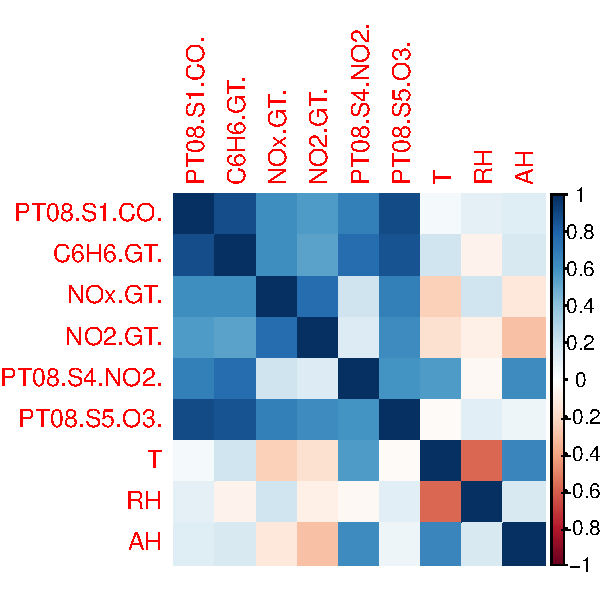
\includegraphics{STA202_report_files/figure-latex/figs-1} 

}

\caption{\label{fig:figs}Matrice de corrélation des variables observées}\label{fig:figs}
\end{figure}

\hypertarget{analyse-en-suxe9rie-temporelle}{%
\subsection{Analyse en série
temporelle}\label{analyse-en-suxe9rie-temporelle}}

L'observation des différentes concentration moyennes périodiques, ainsi
que des séries temporelles elles-mêmes montre un comportement très
similaires entre l'ensemble des gas, si ce n'est pour le Nox.GT dont le
comportement varie. Les émissions hebdomadaires semblent ainsi
inversées, avec un pic d'émissions les lundis et dimanches contre des
pics d'émission en milieu de semaine pour les autres gas. Il en est de
même pour les émissions horaires, avec plus d'émissions tôt le matin
(vers 5h) contre des émissions plus présentes au milieu de la journée
avec les autres gas. Ceci pourrait être expliqué par le fait que les
émissions de ce gaz soient majoritairement dues aux émissions de
transports. Ainsi, les livraisons des magasins par les camions
transporteurs, qui se font en début de semaine et tôt le matin, peuvent
expliquer ces émissions différentes.

\begin{figure}

{\centering 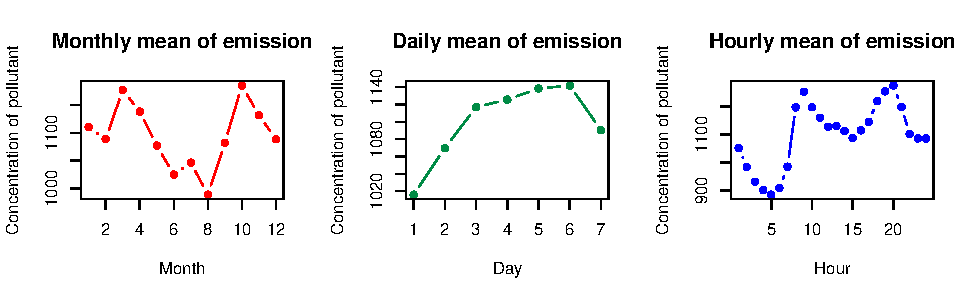
\includegraphics{STA202_report_files/figure-latex/PT08.CO-1} 

}

\caption{\label{fig:PT08.CO} Concentrations moyennes périodiques PT08.CO}\label{fig:PT08.CO}
\end{figure}

\begin{figure}
  \centering
  \includegraphics[height=3cm]{Nox}
  \caption{Concentrations moyennes périodiques NOx.GT}
\end{figure}

La plupart des gaz ayant un comportement similaire, on choisira par la
suite de ne travailler que sur la série temporelle associée à la
concentration de PT08.CO.

\hypertarget{moduxe9lisation-des-donnuxe9es}{%
\section{Modélisation des
données}\label{moduxe9lisation-des-donnuxe9es}}

Pour l'analyse de la série temporelle, nous allons effectuer une
décomposition de la série en tendance, saisonnalité.

Avant de nous attaquer à cette décomposition, une bonne pratique dans
des travaux liés au Machine Learning et aux statistiques est de
normaliser les données. Ceci peut être utile surtout lorsque l'on
souhaite comparer cette série temporelle avec d'autres séries
temporelles qui ne seraient pas de la même échelle.

\begin{Shaded}
\begin{Highlighting}[]
\NormalTok{X}\OtherTok{\textless{}{-}}\NormalTok{(air\_data}\SpecialCharTok{$}\NormalTok{PT08.S1.CO. }\SpecialCharTok{{-}} \FunctionTok{mean}\NormalTok{(air\_data}\SpecialCharTok{$}\NormalTok{PT08.S1.CO.))}\SpecialCharTok{/}\FunctionTok{sd}\NormalTok{(air\_data}\SpecialCharTok{$}\NormalTok{PT08.S1.CO.)}
\NormalTok{X}\OtherTok{\textless{}{-}}\FunctionTok{xts}\NormalTok{(X,}\AttributeTok{order.by=}\NormalTok{Date\_air)}
\end{Highlighting}
\end{Shaded}

\hypertarget{tendances}{%
\subsection{Tendances}\label{tendances}}

Notre série temporelle ne semble à première vue pas comporter de
composante tendancielle. Néanmoins, en zoomant sur sa figure, on observe
des intervalles sur lesquelles elle admet des tendances locales. L'objet
de cette partie sera donc d'extraire ces tendances locales. Nous allons
faire appel à plusieurs méthodes pour annalyser la tendance et la
saisonnalité. Parmi ces méthodes, nous nous intéresserons à la
regression linéaire, la moyenne mobile, la convolution avec un noyau
gaussien, la regression sur une base de splines, la regression par
polynômes locaux.

Pour prédire nos données à l'aides de modèles, il faut d'abord que l'on
sépare notre série temporelle en deux parties. Une partie utilisée pour
l'entraînement des modèles, et une utilisée pour déterminer leur
efficacité.

\begin{Shaded}
\begin{Highlighting}[]
\NormalTok{n }\OtherTok{\textless{}{-}} \FunctionTok{length}\NormalTok{(Date\_air)}
\NormalTok{n.train }\OtherTok{=} \FunctionTok{as.integer}\NormalTok{(}\DecValTok{70}\SpecialCharTok{*}\NormalTok{n}\SpecialCharTok{/}\DecValTok{100}\NormalTok{)}
\NormalTok{X.train }\OtherTok{=}\NormalTok{ X[}\DecValTok{1}\SpecialCharTok{:}\NormalTok{n.train]}
\NormalTok{X.test }\OtherTok{=}\NormalTok{ X[(n.train}\SpecialCharTok{+}\DecValTok{1}\NormalTok{)}\SpecialCharTok{:}\NormalTok{n]}
\NormalTok{X }\OtherTok{\textless{}{-}}\NormalTok{ X.train}
\NormalTok{Date\_air.train }\OtherTok{=}\NormalTok{ Date\_air[}\DecValTok{1}\SpecialCharTok{:}\NormalTok{n.train]}
\end{Highlighting}
\end{Shaded}

\hypertarget{ruxe9gression-linuxe9aire}{%
\subsubsection{Régression linéaire}\label{ruxe9gression-linuxe9aire}}

\begin{Shaded}
\begin{Highlighting}[]
\NormalTok{t }\OtherTok{\textless{}{-}} \FunctionTok{c}\NormalTok{(}\DecValTok{1}\SpecialCharTok{:}\NormalTok{n.train)}

\NormalTok{reg}\FloatTok{.1} \OtherTok{\textless{}{-}} \FunctionTok{lm}\NormalTok{(X}\SpecialCharTok{\textasciitilde{}}\NormalTok{t)}
\NormalTok{reg}\FloatTok{.2} \OtherTok{\textless{}{-}} \FunctionTok{lm}\NormalTok{(X}\SpecialCharTok{\textasciitilde{}}\NormalTok{t}\SpecialCharTok{+}\FunctionTok{I}\NormalTok{(t}\SpecialCharTok{\^{}}\DecValTok{2}\NormalTok{))}
\NormalTok{reg}\FloatTok{.3} \OtherTok{\textless{}{-}} \FunctionTok{lm}\NormalTok{(X}\SpecialCharTok{\textasciitilde{}}\NormalTok{t}\SpecialCharTok{+}\FunctionTok{I}\NormalTok{(t}\SpecialCharTok{\^{}}\DecValTok{2}\NormalTok{)}\SpecialCharTok{+}\FunctionTok{I}\NormalTok{(t}\SpecialCharTok{\^{}}\DecValTok{3}\NormalTok{))}
\NormalTok{reg}\FloatTok{.4} \OtherTok{\textless{}{-}} \FunctionTok{lm}\NormalTok{(X}\SpecialCharTok{\textasciitilde{}}\NormalTok{t}\SpecialCharTok{+}\FunctionTok{I}\NormalTok{(t}\SpecialCharTok{\^{}}\DecValTok{2}\NormalTok{)}\SpecialCharTok{+}\FunctionTok{I}\NormalTok{(t}\SpecialCharTok{\^{}}\DecValTok{3}\NormalTok{)}\SpecialCharTok{+}\FunctionTok{I}\NormalTok{(t}\SpecialCharTok{\^{}}\DecValTok{4}\NormalTok{))}
\NormalTok{reg}\FloatTok{.5} \OtherTok{\textless{}{-}} \FunctionTok{lm}\NormalTok{(X}\SpecialCharTok{\textasciitilde{}}\NormalTok{t}\SpecialCharTok{+}\FunctionTok{I}\NormalTok{(t}\SpecialCharTok{\^{}}\DecValTok{2}\NormalTok{)}\SpecialCharTok{+}\FunctionTok{I}\NormalTok{(t}\SpecialCharTok{\^{}}\DecValTok{3}\NormalTok{)}\SpecialCharTok{+}\FunctionTok{I}\NormalTok{(t}\SpecialCharTok{\^{}}\DecValTok{4}\NormalTok{)}\SpecialCharTok{+}\FunctionTok{I}\NormalTok{(t}\SpecialCharTok{\^{}}\DecValTok{5}\NormalTok{))}

\NormalTok{y.chap.lm}\FloatTok{.1} \OtherTok{\textless{}{-}} \FunctionTok{xts}\NormalTok{(reg}\FloatTok{.1}\SpecialCharTok{$}\NormalTok{fitted, }\AttributeTok{order.by =}\NormalTok{ Date\_air.train)}
\NormalTok{y.chap.lm}\FloatTok{.2} \OtherTok{\textless{}{-}} \FunctionTok{xts}\NormalTok{(reg}\FloatTok{.2}\SpecialCharTok{$}\NormalTok{fitted, }\AttributeTok{order.by =}\NormalTok{ Date\_air.train)}
\NormalTok{y.chap.lm}\FloatTok{.3} \OtherTok{\textless{}{-}} \FunctionTok{xts}\NormalTok{(reg}\FloatTok{.3}\SpecialCharTok{$}\NormalTok{fitted, }\AttributeTok{order.by =}\NormalTok{ Date\_air.train)}
\NormalTok{y.chap.lm}\FloatTok{.4} \OtherTok{\textless{}{-}} \FunctionTok{xts}\NormalTok{(reg}\FloatTok{.4}\SpecialCharTok{$}\NormalTok{fitted, }\AttributeTok{order.by =}\NormalTok{ Date\_air.train)}
\NormalTok{y.chap.lm}\FloatTok{.5} \OtherTok{\textless{}{-}} \FunctionTok{xts}\NormalTok{(reg}\FloatTok{.5}\SpecialCharTok{$}\NormalTok{fitted, }\AttributeTok{order.by =}\NormalTok{ Date\_air.train)}
\end{Highlighting}
\end{Shaded}

\begin{figure}

{\centering 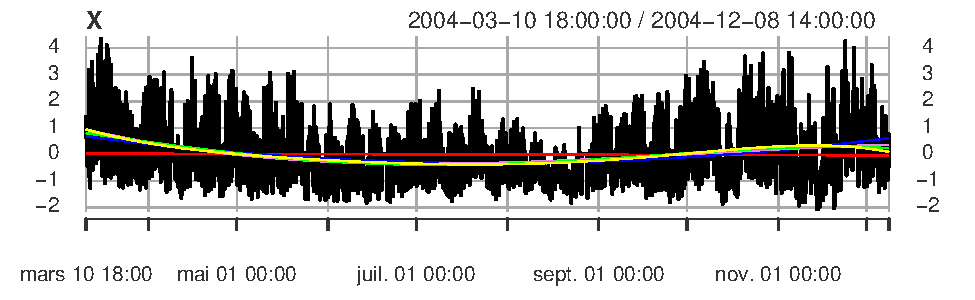
\includegraphics{STA202_report_files/figure-latex/lm_fig-1} 

}

\caption{\label{fig:lm_fig} Régression linéaire ; d°1:rouge, d°2:bleu, d°3:violet, d°4:vert, d°5:jaune}\label{fig:lm_fig}
\end{figure}

On observe sur la figure \ref{fig:lm_fig} que la régression linéaire sur
les droites nous affichent une pente quasi nulle devant l'amplitude des
données. Pour l'ordre 2, on remarque qu'il y a un léger comportement
convexe sur les données.

La régression à l'ordre 4 semble bien capturer le comportement
basse-fréquence de la série, sans montrer d'abérration comme le fait le
modèle d'ordre 5 vers la fin du graphe, en remontant. Pour éviter le
surapprentissage, un modèle à l'ordre 4 semble raisonnable.

En soustrayant à X la tendance estimée, on obtient un signal qui est
bien centré en 0.

\begin{figure}

{\centering 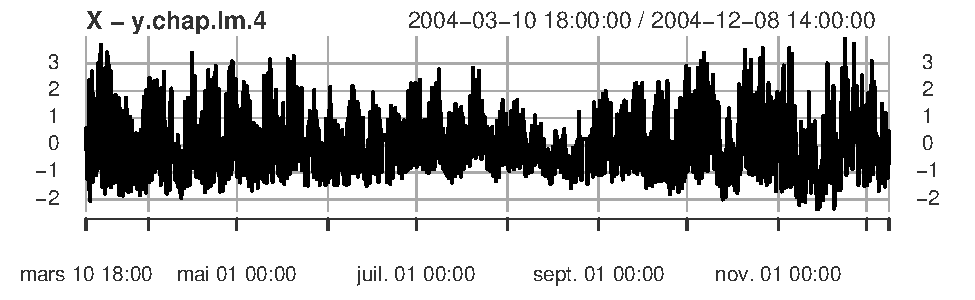
\includegraphics{STA202_report_files/figure-latex/X.detrend.lm-1} 

}

\caption{\label{fig:X.detrend.lm} X.detrend lm}\label{fig:X.detrend.lm}
\end{figure}

\hypertarget{moyenne-mobile}{%
\subsubsection{Moyenne mobile}\label{moyenne-mobile}}

La moyenne mobile peut être utilisée pour capter la tendance de notre
série. Notre série étant périodique de période 24h, il sera important
d'ajuster la fenêtre correctement pour filtrer la saisonnalité.

\begin{Shaded}
\begin{Highlighting}[]
\NormalTok{l }\OtherTok{\textless{}{-}} \DecValTok{24}
\NormalTok{MA.trend }\OtherTok{\textless{}{-}}\NormalTok{ stats}\SpecialCharTok{::}\FunctionTok{filter}\NormalTok{(X, }\AttributeTok{filter=}\FunctionTok{array}\NormalTok{(}\DecValTok{1}\SpecialCharTok{/}\NormalTok{l,}\AttributeTok{dim=}\NormalTok{l),}
                  \AttributeTok{method =} \FunctionTok{c}\NormalTok{(}\StringTok{"convolution"}\NormalTok{),}
                  \AttributeTok{sides =} \DecValTok{2}\NormalTok{, }\AttributeTok{circular =}\NormalTok{ F)}
\NormalTok{MA.trend }\OtherTok{\textless{}{-}} \FunctionTok{xts}\NormalTok{(MA.trend, }\AttributeTok{order.by=}\NormalTok{Date\_air.train)}
\NormalTok{X.detrend }\OtherTok{\textless{}{-}}\NormalTok{ X }\SpecialCharTok{{-}}\NormalTok{ MA.trend}
\end{Highlighting}
\end{Shaded}

\begin{figure}

{\centering 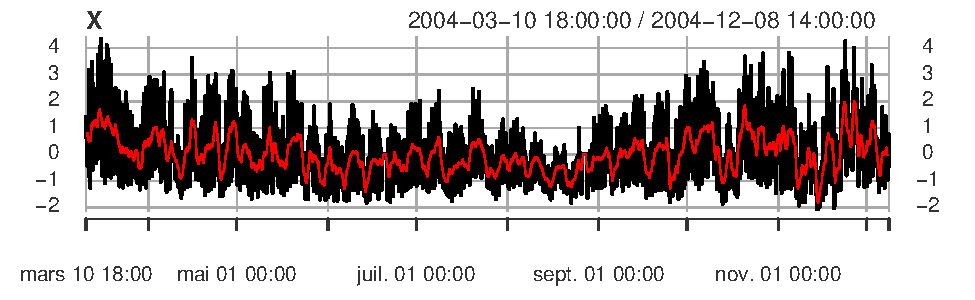
\includegraphics{STA202_report_files/figure-latex/ma-1} 

}

\caption{\label{fig:ma} Moyenne mobile de fenêtre l=24}\label{fig:ma}
\end{figure}

L'utilisation de la moyenne mobile calcule une tendance avec des
fréquences beaucoup plus hautes et semble tout de même. Néamoins, la
série corrigée de la tendance reste bien centrée.

\hypertarget{convolution-sur-un-noyau-gaussien}{%
\subsubsection{Convolution sur un noyau
gaussien}\label{convolution-sur-un-noyau-gaussien}}

\begin{Shaded}
\begin{Highlighting}[]
\NormalTok{h}\OtherTok{\textless{}{-}}\DecValTok{10000}

\NormalTok{x}\OtherTok{\textless{}{-}}\FunctionTok{seq}\NormalTok{(}\DecValTok{1}\NormalTok{,}\FunctionTok{max}\NormalTok{(t),}\AttributeTok{length=}\NormalTok{n.train)}

\NormalTok{noyau }\OtherTok{\textless{}{-}} \ControlFlowTok{function}\NormalTok{(x)\{}\FunctionTok{dnorm}\NormalTok{(x}\SpecialCharTok{{-}}\NormalTok{t,}\DecValTok{0}\NormalTok{,}\AttributeTok{sd=}\FunctionTok{sqrt}\NormalTok{(h}\SpecialCharTok{/}\DecValTok{2}\NormalTok{))}\SpecialCharTok{/}\FunctionTok{sum}\NormalTok{(}\FunctionTok{dnorm}\NormalTok{(x}\SpecialCharTok{{-}}\NormalTok{t,}\DecValTok{0}\NormalTok{,}\AttributeTok{sd=}\FunctionTok{sqrt}\NormalTok{(h}\SpecialCharTok{/}\DecValTok{2}\NormalTok{)))\}}

\NormalTok{W}\OtherTok{\textless{}{-}}\FunctionTok{matrix}\NormalTok{(}\FunctionTok{unlist}\NormalTok{(}\FunctionTok{lapply}\NormalTok{(x,noyau)),}\AttributeTok{ncol=}\NormalTok{n.train,}\AttributeTok{nrow=}\NormalTok{n.train,}\AttributeTok{byrow=}\NormalTok{F)}

\NormalTok{ychap.kernel}\OtherTok{\textless{}{-}}\FunctionTok{colSums}\NormalTok{(}\FunctionTok{as.numeric}\NormalTok{(X)}\SpecialCharTok{*}\NormalTok{W)}
\NormalTok{ychap.kernel}\OtherTok{\textless{}{-}}\FunctionTok{xts}\NormalTok{(ychap.kernel,}\AttributeTok{order.by=}\NormalTok{Date\_air.train)}
\end{Highlighting}
\end{Shaded}

\begin{figure}

{\centering 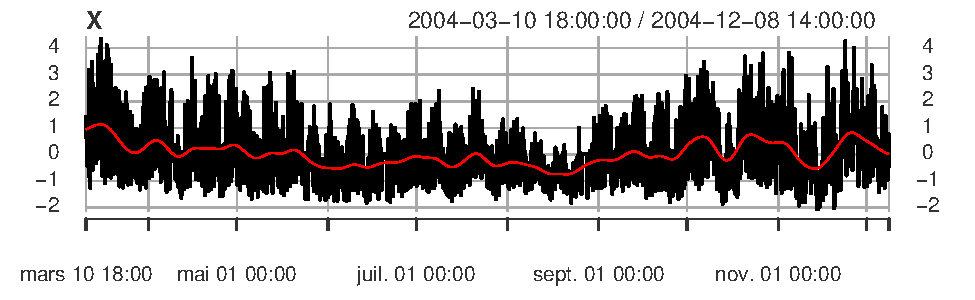
\includegraphics{STA202_report_files/figure-latex/kernel-1} 

}

\caption{\label{fig:kernel} Noyau gaussien, fenêtre h=10000}\label{fig:kernel}
\end{figure}

L'utilisation du noyau gaussien avec un paramètre h raisonnable semble
donner un bon compromis entre la moyenne mobile de fenêtre 24, et la
régression linéaire.

\hypertarget{ruxe9gression-sur-base-de-splines}{%
\subsubsection{Régression sur base de
splines}\label{ruxe9gression-sur-base-de-splines}}

\begin{Shaded}
\begin{Highlighting}[]
\NormalTok{g }\OtherTok{\textless{}{-}} \FunctionTok{gam}\NormalTok{(X}\SpecialCharTok{\textasciitilde{}}\FunctionTok{s}\NormalTok{(t, }\AttributeTok{k=}\DecValTok{5}\NormalTok{))}
\NormalTok{ychap.gam}\OtherTok{\textless{}{-}}\FunctionTok{xts}\NormalTok{(g}\SpecialCharTok{$}\NormalTok{fitted,}\AttributeTok{order.by=}\NormalTok{Date\_air.train)}
\end{Highlighting}
\end{Shaded}

\begin{figure}

{\centering 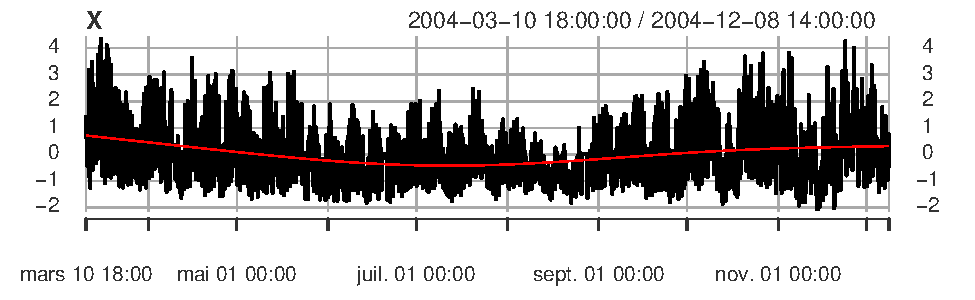
\includegraphics{STA202_report_files/figure-latex/splines-1} 

}

\caption{\label{fig:splines} Base de splines, k=5}\label{fig:splines}
\end{figure}

La régression sur la base de spline montre un très bon résultat, les
basses fréquences ont bien été extraites du signal.

\hypertarget{ruxe9gression-par-polynuxf4mes-locaux}{%
\subsubsection{Régression par polynômes
locaux}\label{ruxe9gression-par-polynuxf4mes-locaux}}

\begin{Shaded}
\begin{Highlighting}[]
\NormalTok{X }\OtherTok{\textless{}{-}} \FunctionTok{xts}\NormalTok{(X,}\AttributeTok{order.by=}\NormalTok{Date\_air.train)}
\NormalTok{lo }\OtherTok{\textless{}{-}} \FunctionTok{loess}\NormalTok{(X}\SpecialCharTok{\textasciitilde{}}\NormalTok{t, }\AttributeTok{degree=}\DecValTok{2}\NormalTok{, }\AttributeTok{span=}\FloatTok{0.7}\NormalTok{)}
\NormalTok{ychap.lo }\OtherTok{\textless{}{-}} \FunctionTok{xts}\NormalTok{(lo}\SpecialCharTok{$}\NormalTok{fitted,}\AttributeTok{order.by=}\NormalTok{Date\_air.train)}
\end{Highlighting}
\end{Shaded}

\begin{figure}

{\centering 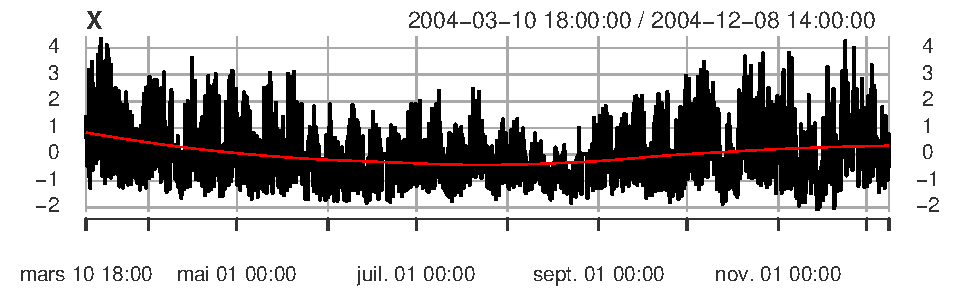
\includegraphics{STA202_report_files/figure-latex/polynoms-1} 

}

\caption{\label{fig:polynoms} Polynômes locaux}\label{fig:polynoms}
\end{figure}

Un degré adapté pour les polynômes locaux nous permet aussi d'extraire
les basses fréquences du signal.

On choisira finalement arbitrairement de modéliser la tendance de la
série à l'aide de sa décomposition sur la base de splines.

Le signal ainsi corrigé est le suivant :

\begin{figure}

{\centering 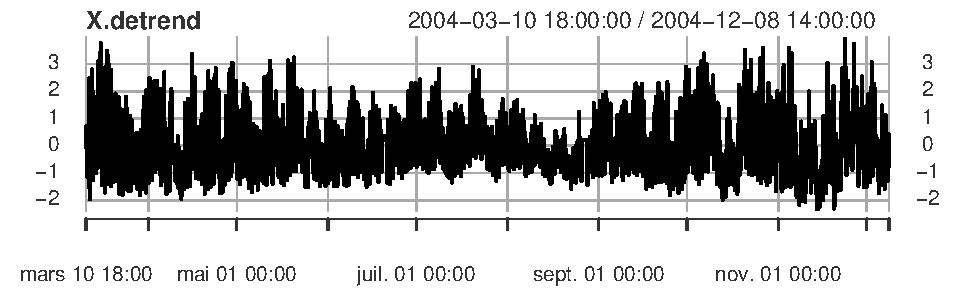
\includegraphics{STA202_report_files/figure-latex/splines.center-1} 

}

\caption{\label{fig:splines.center} Signal centré}\label{fig:splines.center}
\end{figure}

\hypertarget{saisonnalituxe9}{%
\subsection{Saisonnalité}\label{saisonnalituxe9}}

Pour étudier la saisonnalité de nos données nous allons regarder
l'autocorélogramme de notre série.

\begin{Shaded}
\begin{Highlighting}[]
\FunctionTok{Acf}\NormalTok{(X.detrend,}\AttributeTok{lag.max=}\DecValTok{200}\NormalTok{)}
\end{Highlighting}
\end{Shaded}

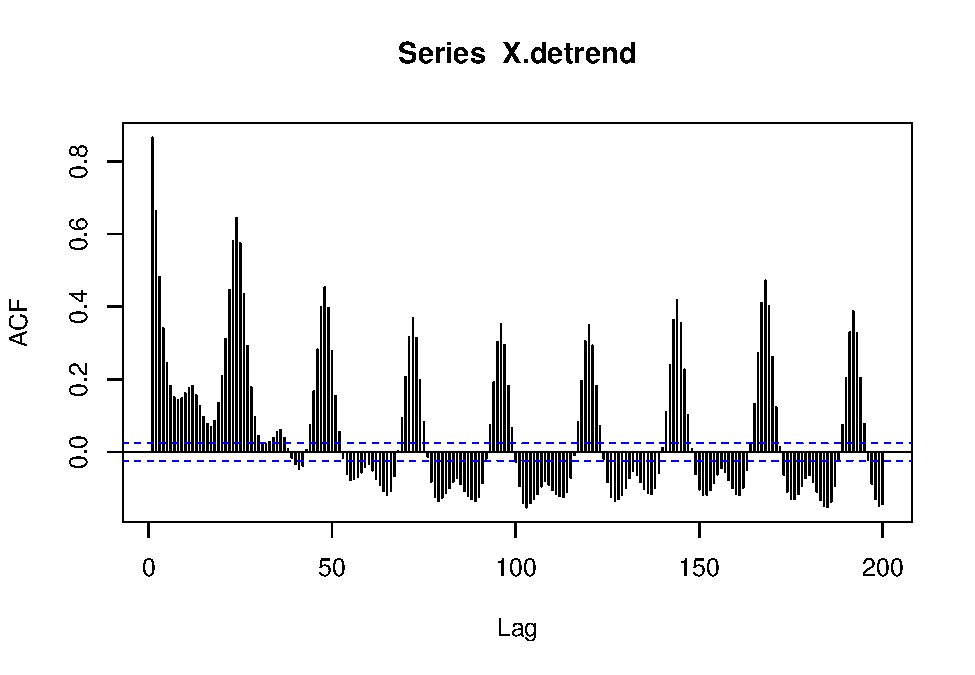
\includegraphics{STA202_report_files/figure-latex/unnamed-chunk-19-1.pdf}

L'oscillation de l'ACF avec des pics réguliers toutes les 24h (et même
12h) montre l'existence d'une saisonnalité journalière dans nos données.
L'existance de cette saisonnalité dément la stationnarité de la série
temporelle. Ceci est d'autant plus justifié qu'il n'y a pas de
décroissance exponentielle. Ceci peut également être vérifié en
utilisant le test ADF (Augmented Dickey-Fuller), qui teste l'hypothèse
nulle suivante :
\[(H_0): \text{La série temporelle est non stationnaire}\] Le test ADF
affiche une p-value de 0.99, ce qui est bien au dessus de 0.05. On ne
peut donc pas rejeter l'hypothèse nulle. La série temporelle est donc
non stationnaire.

\begin{Shaded}
\begin{Highlighting}[]
\FunctionTok{adf.test}\NormalTok{(X.detrend)}
\end{Highlighting}
\end{Shaded}

\hypertarget{extraction-de-la-saisonnalituxe9-par-duxe9composition-en-suxe9rie-de-fourier}{%
\subsubsection{Extraction de la saisonnalité par décomposition en série
de
fourier}\label{extraction-de-la-saisonnalituxe9-par-duxe9composition-en-suxe9rie-de-fourier}}

On effectue une régression linéaire sur une base de fourier associée à
la pulsation de fréquence 1/24. L'affichage de la figure
\ref{fig:saisonnalite} montre bien un signal périodique, qui semble
représenter la saisonnalité de la série temporelle. Néanmoins,
l'amplitude de ce signal est relativement faible, ce qui contredit
l'analyse que l'on a fait de l'ACF\ldots{}

\begin{Shaded}
\begin{Highlighting}[]
\NormalTok{w}\OtherTok{=}\DecValTok{2}\SpecialCharTok{*}\NormalTok{pi}\SpecialCharTok{/}\DecValTok{24}
\NormalTok{fourier}\OtherTok{\textless{}{-}}\FunctionTok{cbind}\NormalTok{(}\FunctionTok{cos}\NormalTok{(w}\SpecialCharTok{*}\NormalTok{t), }\FunctionTok{sin}\NormalTok{(w}\SpecialCharTok{*}\NormalTok{t))}
\NormalTok{K}\OtherTok{\textless{}{-}}\DecValTok{30}
\ControlFlowTok{for}\NormalTok{(i }\ControlFlowTok{in} \FunctionTok{c}\NormalTok{(}\DecValTok{2}\SpecialCharTok{:}\NormalTok{K))}
\NormalTok{\{}
\NormalTok{  fourier}\OtherTok{\textless{}{-}}\FunctionTok{cbind}\NormalTok{(fourier,}\FunctionTok{cos}\NormalTok{(i}\SpecialCharTok{*}\NormalTok{w}\SpecialCharTok{*}\NormalTok{t), }\FunctionTok{sin}\NormalTok{(i}\SpecialCharTok{*}\NormalTok{w}\SpecialCharTok{*}\NormalTok{t))}
\NormalTok{\}}

\NormalTok{reg}\OtherTok{\textless{}{-}}\FunctionTok{lm}\NormalTok{(X.detrend}\SpecialCharTok{\textasciitilde{}}\NormalTok{fourier[,}\DecValTok{1}\SpecialCharTok{:}\NormalTok{K]}\SpecialCharTok{{-}}\DecValTok{1}\NormalTok{)}
\NormalTok{ychap.lm.season}\OtherTok{\textless{}{-}}\FunctionTok{xts}\NormalTok{(}\FunctionTok{as.numeric}\NormalTok{(reg}\SpecialCharTok{$}\NormalTok{fitted),}\AttributeTok{order.by=}\NormalTok{Date\_air.train)}
\end{Highlighting}
\end{Shaded}

Le résidu devient finalement le suivant.

\begin{figure}

{\centering 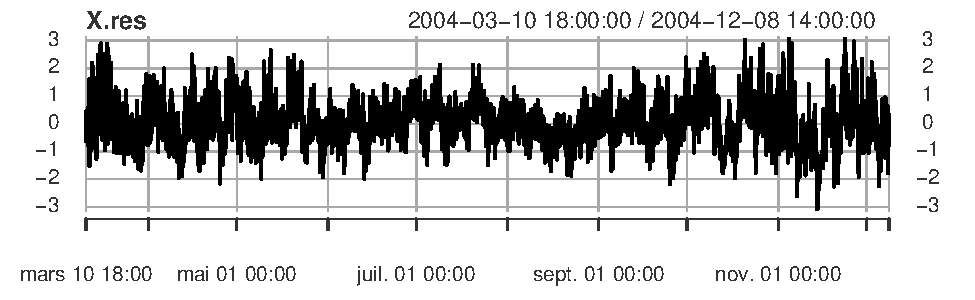
\includegraphics{STA202_report_files/figure-latex/residu-1} 

}

\caption{\label{fig:residu} Résidu}\label{fig:residu}
\end{figure}

\hypertarget{diffuxe9rentiation}{%
\subsubsection{Différentiation}\label{diffuxe9rentiation}}

Plutôt que d'utiliser la méthode précédente pour éliminer la
saisonnalité, nous allons procéder à une différentiation.

On va pouvoir se rapprocher d'un comportement stationnaire être atteinte
en différenciant la série temporelle. La saisonnalité journalière nous
pousse ainsi à différencier nos données avec un lag de 24 via
l'opérateur \(1-L^{24}\). Nous affichons maintenant l'autocorrélogramme
de notre série différenciée :

\begin{Shaded}
\begin{Highlighting}[]
\NormalTok{X.detrend.diff }\OtherTok{\textless{}{-}} \FunctionTok{na\_mean}\NormalTok{(}\FunctionTok{diff}\NormalTok{(X.detrend, }\AttributeTok{lag=}\DecValTok{24}\NormalTok{, }\AttributeTok{differences=}\DecValTok{1}\NormalTok{))}
\end{Highlighting}
\end{Shaded}

On obtient un graphique satisfaisant avec une décroissance vers zéro,
mais cette décroissance est très lente\ldots{} On souhaite maintenant
déduire les plages de paramètres possibles pour un modèle \(ARMA(p,q)\)
du résidu. Pour ce faire, on étudie l'autocorrélogramme et
l'autocorrélogramme partiel de la série différenciée.

\begin{Shaded}
\begin{Highlighting}[]
\FunctionTok{par}\NormalTok{(}\FunctionTok{c}\NormalTok{(}\DecValTok{1}\NormalTok{, }\DecValTok{2}\NormalTok{))}
\end{Highlighting}
\end{Shaded}

\begin{verbatim}
## Warning in par(c(1, 2)): argument 1 does not name a graphical parameter
\end{verbatim}

\begin{verbatim}
## NULL
\end{verbatim}

\begin{Shaded}
\begin{Highlighting}[]
\FunctionTok{Acf}\NormalTok{(X.detrend.diff,}\AttributeTok{lag.max=}\DecValTok{50}\NormalTok{)}
\end{Highlighting}
\end{Shaded}

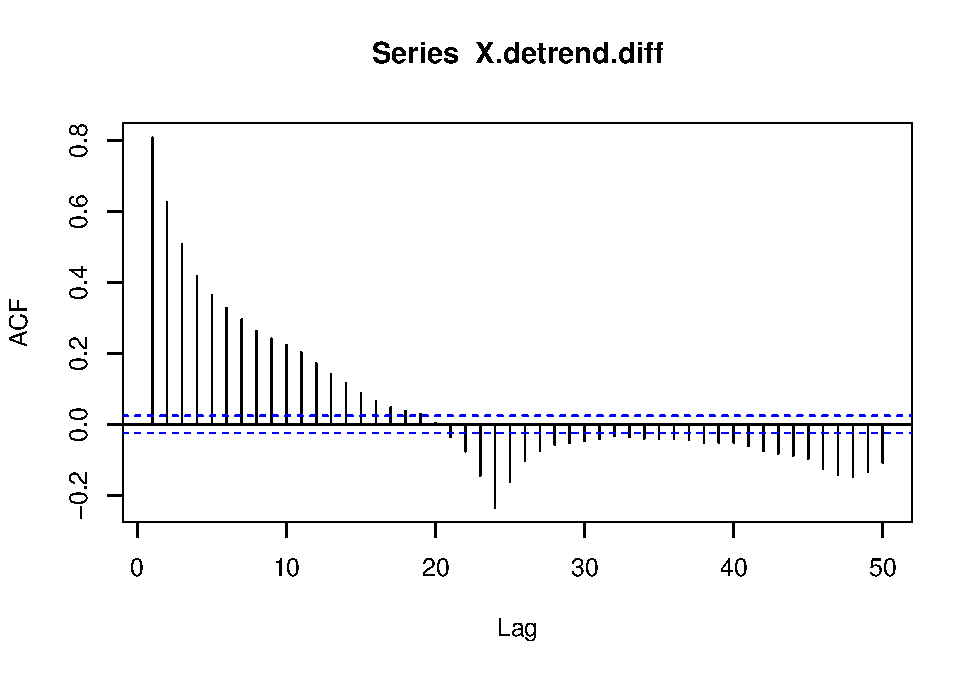
\includegraphics{STA202_report_files/figure-latex/unnamed-chunk-23-1.pdf}

\begin{Shaded}
\begin{Highlighting}[]
\FunctionTok{Pacf}\NormalTok{(X.detrend.diff, }\AttributeTok{lag.max=}\DecValTok{50}\NormalTok{)}
\end{Highlighting}
\end{Shaded}

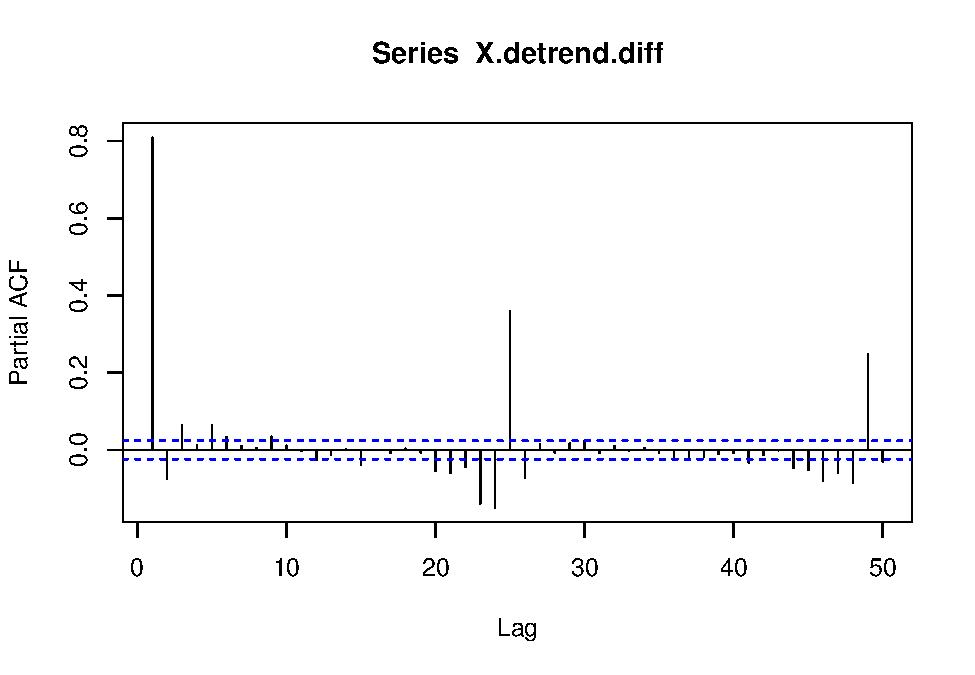
\includegraphics{STA202_report_files/figure-latex/unnamed-chunk-23-2.pdf}

On va donc modéliser notre résidu par un modèle ARMA. Il nous reste à
choisir les paramètres p et q. Pour le paramètre, on note que
l'autocorrélogramme partiel possède un pic au lag=1,2,3 qui sont
significatifs. Il y a également des pics significatifs entre 20 et 25
mais le nombre de pics non significatifs avant ces lags nous fait penser
que l'on peut se restreindre aux 3 premiers, c'est à dire pmax=3.
L'étude de l'autocorrélogramme nous apporte moins d'informations car les
pics sont significatifs jusqu'aux lags 40 au moins. Cependant, les pics
décroissent exponentiellement jusq'au lag 20, on peut donc penser
prendre qmax=20. Il nous faut ensuite tester tous les modèles et choisir
le meilleur selon le critère AIC. En suivant cette méthodologie, c'est
le modèle ARMA(3, 0, 20) qui possède le plus faible AIC parmis
l'ensemble des modèles calculés, avec un AIC de 8115.5.

Bien que le résidu semble être gaussien, le test de Ljung-Box nous
indique que ce n'est pas le cas. Ceci est sûrement du à la persistance
de la saisonnalité, qui malgré une différentiation (et même plus lors de
nos tests), semble ne pas vouloir disparaître.

\hypertarget{prediction}{%
\section{Prediction}\label{prediction}}

La prédiction sur un jeu de données tests va permettre d'évaluer les
modèles. On procèdera ici à la prédiction par le modèle ARMA calculé
précédemment, mais aussi à un modèle de prédiction par lissage
exponentiel.

\hypertarget{moduxe8le-arma}{%
\subsection{Modèle ARMA}\label{moduxe8le-arma}}

\begin{Shaded}
\begin{Highlighting}[]
\NormalTok{n.test }\OtherTok{=}\NormalTok{ n }\SpecialCharTok{{-}}\NormalTok{ n.train}
\NormalTok{arma.forecast }\OtherTok{\textless{}{-}} \FunctionTok{predict}\NormalTok{(model, }\AttributeTok{n.ahead =}\NormalTok{ n.test, }\AttributeTok{se.fit =}\NormalTok{F)}
\FunctionTok{plot}\NormalTok{(arma.forecast)}
\end{Highlighting}
\end{Shaded}

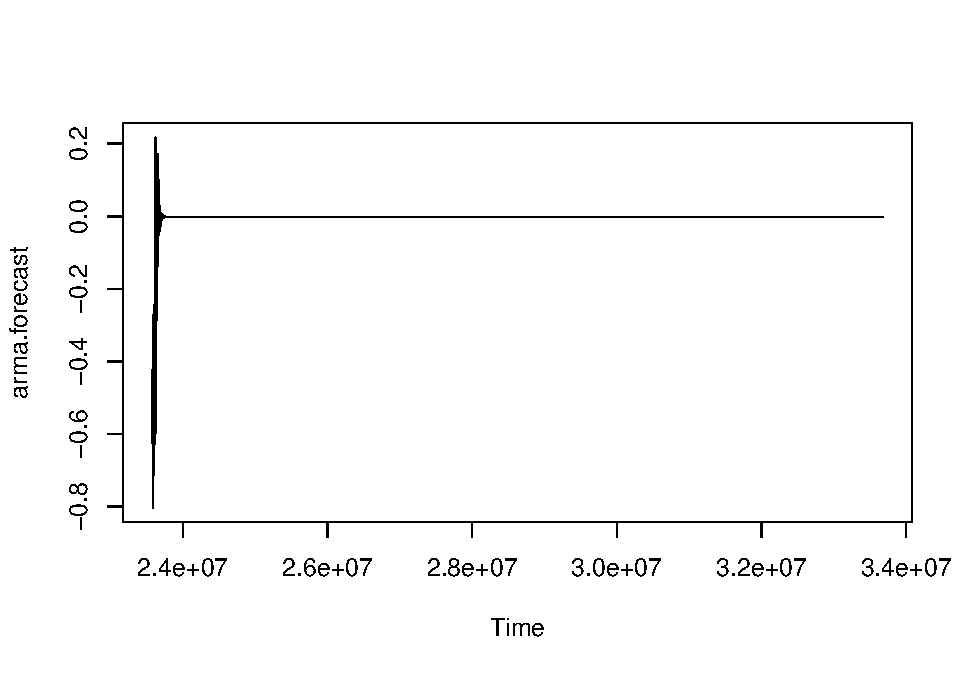
\includegraphics{STA202_report_files/figure-latex/ARMA.predict-1.pdf}

\begin{Shaded}
\begin{Highlighting}[]
\FunctionTok{plot}\NormalTok{(X.detrend.diff,}\AttributeTok{xlim=}\FunctionTok{c}\NormalTok{(}\DecValTok{1}\NormalTok{,}\FunctionTok{nrow}\NormalTok{(data)}\SpecialCharTok{+}\NormalTok{n.test))}
\end{Highlighting}
\end{Shaded}

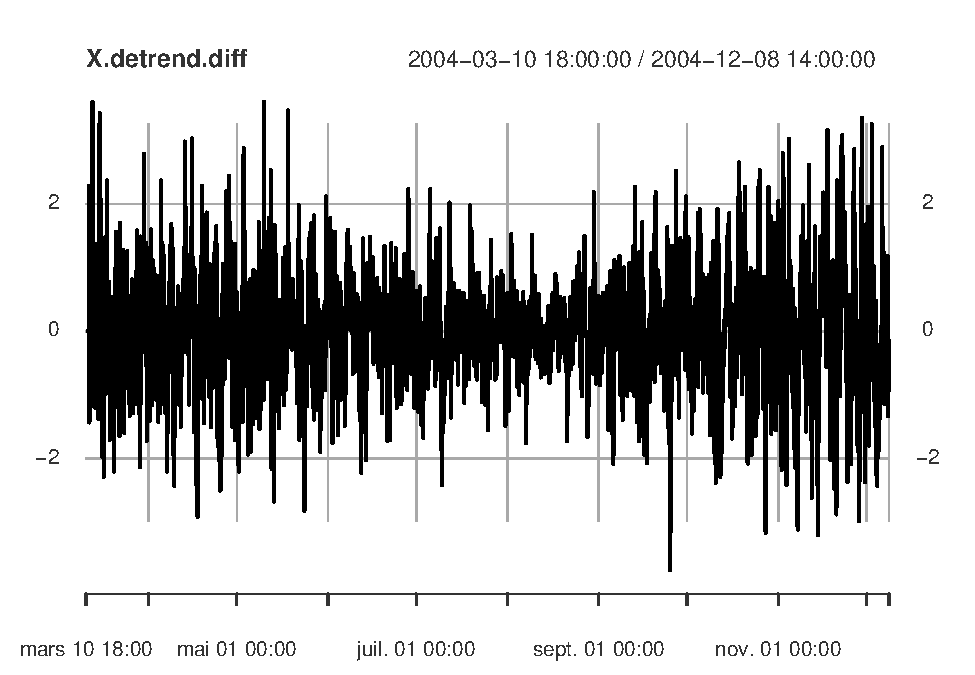
\includegraphics{STA202_report_files/figure-latex/ARMA.predict-2.pdf}

Les problèmes que l'on a eu avec le modèle ARMA du résidu se répercutent
ici\ldots{}

\hypertarget{lissage-exponentiel}{%
\subsection{Lissage exponentiel}\label{lissage-exponentiel}}

\begin{Shaded}
\begin{Highlighting}[]
\NormalTok{ses.model }\OtherTok{\textless{}{-}}\NormalTok{ forecast}\SpecialCharTok{::}\FunctionTok{ses}\NormalTok{(X.train, }\AttributeTok{alpha=}\FloatTok{0.99}\NormalTok{, }\AttributeTok{h=}\NormalTok{n.test)}
\NormalTok{forecast.ses }\OtherTok{\textless{}{-}}\NormalTok{ forecast}\SpecialCharTok{::}\FunctionTok{forecast}\NormalTok{(ses.model, n.test)}
\FunctionTok{par}\NormalTok{(}\AttributeTok{mfrow=}\FunctionTok{c}\NormalTok{(}\DecValTok{1}\NormalTok{, }\DecValTok{2}\NormalTok{))}
\FunctionTok{plot}\NormalTok{(forecast.ses, }\AttributeTok{ylim=}\FunctionTok{c}\NormalTok{(}\SpecialCharTok{{-}}\DecValTok{3}\NormalTok{, }\DecValTok{3}\NormalTok{))}
\FunctionTok{plot}\NormalTok{(X.detrend.diff)}
\end{Highlighting}
\end{Shaded}

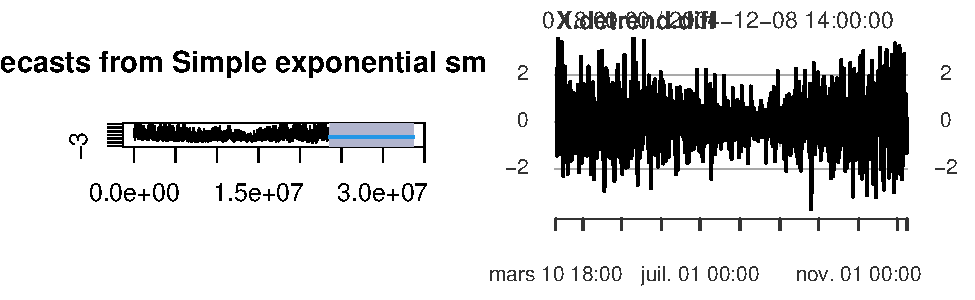
\includegraphics{STA202_report_files/figure-latex/SES-1.pdf} Le lissage
exponentiel donne une estimation à l'ordre 0 des données.

\hypertarget{inversion}{%
\subsection{Inversion}\label{inversion}}

Une fois que le résidu a été prédit avec un bon modèle, il ne resterait
plus qu'à inverser les étapes de stationnarisation. En appliquant
l'inverse de la différentiation de période 24, à l'aide de la fonction
\(invdiff\), puis en ajoutant la composante saisonnière prédite sur
lintervalle choisi. Il ne resterait alors plus qu'à dénormaliser en
mumtipliant par la déviation standard et en ajoutant la moyenne.

\end{document}
